% Options for packages loaded elsewhere
\PassOptionsToPackage{unicode}{hyperref}
\PassOptionsToPackage{hyphens}{url}
%
\documentclass[
  14pt,
  ignorenonframetext,
  aspectratio=169,
]{beamer}
\usepackage{pgfpages}
\setbeamertemplate{caption}[numbered]
\setbeamertemplate{caption label separator}{: }
\setbeamercolor{caption name}{fg=normal text.fg}
\beamertemplatenavigationsymbolsempty
% Prevent slide breaks in the middle of a paragraph
\widowpenalties 1 10000
\raggedbottom

\usepackage{amsmath,amssymb}
\usepackage{iftex}
\ifPDFTeX
  \usepackage[T1]{fontenc}
  \usepackage[utf8]{inputenc}
  \usepackage{textcomp} % provide euro and other symbols
\else % if luatex or xetex
  \usepackage{unicode-math}
  \defaultfontfeatures{Scale=MatchLowercase}
  \defaultfontfeatures[\rmfamily]{Ligatures=TeX,Scale=1}
\fi
\usepackage{lmodern}
\ifPDFTeX\else  
    % xetex/luatex font selection
\fi
% Use upquote if available, for straight quotes in verbatim environments
\IfFileExists{upquote.sty}{\usepackage{upquote}}{}
\IfFileExists{microtype.sty}{% use microtype if available
  \usepackage[]{microtype}
  \UseMicrotypeSet[protrusion]{basicmath} % disable protrusion for tt fonts
}{}
\makeatletter
\@ifundefined{KOMAClassName}{% if non-KOMA class
  \IfFileExists{parskip.sty}{%
    \usepackage{parskip}
  }{% else
    \setlength{\parindent}{0pt}
    \setlength{\parskip}{6pt plus 2pt minus 1pt}}
}{% if KOMA class
  \KOMAoptions{parskip=half}}
\makeatother
\usepackage{xcolor}
\newif\ifbibliography
\setlength{\emergencystretch}{3em} % prevent overfull lines
\setcounter{secnumdepth}{-\maxdimen} % remove section numbering

\usepackage{color}
\usepackage{fancyvrb}
\newcommand{\VerbBar}{|}
\newcommand{\VERB}{\Verb[commandchars=\\\{\}]}
\DefineVerbatimEnvironment{Highlighting}{Verbatim}{commandchars=\\\{\}}
% Add ',fontsize=\small' for more characters per line
\usepackage{framed}
\definecolor{shadecolor}{RGB}{248,248,248}
\newenvironment{Shaded}{\begin{snugshade}}{\end{snugshade}}
\newcommand{\AlertTok}[1]{\textcolor[rgb]{0.94,0.16,0.16}{#1}}
\newcommand{\AnnotationTok}[1]{\textcolor[rgb]{0.56,0.35,0.01}{\textbf{\textit{#1}}}}
\newcommand{\AttributeTok}[1]{\textcolor[rgb]{0.13,0.29,0.53}{#1}}
\newcommand{\BaseNTok}[1]{\textcolor[rgb]{0.00,0.00,0.81}{#1}}
\newcommand{\BuiltInTok}[1]{#1}
\newcommand{\CharTok}[1]{\textcolor[rgb]{0.31,0.60,0.02}{#1}}
\newcommand{\CommentTok}[1]{\textcolor[rgb]{0.56,0.35,0.01}{\textit{#1}}}
\newcommand{\CommentVarTok}[1]{\textcolor[rgb]{0.56,0.35,0.01}{\textbf{\textit{#1}}}}
\newcommand{\ConstantTok}[1]{\textcolor[rgb]{0.56,0.35,0.01}{#1}}
\newcommand{\ControlFlowTok}[1]{\textcolor[rgb]{0.13,0.29,0.53}{\textbf{#1}}}
\newcommand{\DataTypeTok}[1]{\textcolor[rgb]{0.13,0.29,0.53}{#1}}
\newcommand{\DecValTok}[1]{\textcolor[rgb]{0.00,0.00,0.81}{#1}}
\newcommand{\DocumentationTok}[1]{\textcolor[rgb]{0.56,0.35,0.01}{\textbf{\textit{#1}}}}
\newcommand{\ErrorTok}[1]{\textcolor[rgb]{0.64,0.00,0.00}{\textbf{#1}}}
\newcommand{\ExtensionTok}[1]{#1}
\newcommand{\FloatTok}[1]{\textcolor[rgb]{0.00,0.00,0.81}{#1}}
\newcommand{\FunctionTok}[1]{\textcolor[rgb]{0.13,0.29,0.53}{\textbf{#1}}}
\newcommand{\ImportTok}[1]{#1}
\newcommand{\InformationTok}[1]{\textcolor[rgb]{0.56,0.35,0.01}{\textbf{\textit{#1}}}}
\newcommand{\KeywordTok}[1]{\textcolor[rgb]{0.13,0.29,0.53}{\textbf{#1}}}
\newcommand{\NormalTok}[1]{#1}
\newcommand{\OperatorTok}[1]{\textcolor[rgb]{0.81,0.36,0.00}{\textbf{#1}}}
\newcommand{\OtherTok}[1]{\textcolor[rgb]{0.56,0.35,0.01}{#1}}
\newcommand{\PreprocessorTok}[1]{\textcolor[rgb]{0.56,0.35,0.01}{\textit{#1}}}
\newcommand{\RegionMarkerTok}[1]{#1}
\newcommand{\SpecialCharTok}[1]{\textcolor[rgb]{0.81,0.36,0.00}{\textbf{#1}}}
\newcommand{\SpecialStringTok}[1]{\textcolor[rgb]{0.31,0.60,0.02}{#1}}
\newcommand{\StringTok}[1]{\textcolor[rgb]{0.31,0.60,0.02}{#1}}
\newcommand{\VariableTok}[1]{\textcolor[rgb]{0.00,0.00,0.00}{#1}}
\newcommand{\VerbatimStringTok}[1]{\textcolor[rgb]{0.31,0.60,0.02}{#1}}
\newcommand{\WarningTok}[1]{\textcolor[rgb]{0.56,0.35,0.01}{\textbf{\textit{#1}}}}

\providecommand{\tightlist}{%
  \setlength{\itemsep}{0pt}\setlength{\parskip}{0pt}}\usepackage{longtable,booktabs,array}
\usepackage{calc} % for calculating minipage widths
\usepackage{caption}
% Make caption package work with longtable
\makeatletter
\def\fnum@table{\tablename~\thetable}
\makeatother
\usepackage{graphicx}
\makeatletter
\def\maxwidth{\ifdim\Gin@nat@width>\linewidth\linewidth\else\Gin@nat@width\fi}
\def\maxheight{\ifdim\Gin@nat@height>\textheight\textheight\else\Gin@nat@height\fi}
\makeatother
% Scale images if necessary, so that they will not overflow the page
% margins by default, and it is still possible to overwrite the defaults
% using explicit options in \includegraphics[width, height, ...]{}
\setkeys{Gin}{width=\maxwidth,height=\maxheight,keepaspectratio}
% Set default figure placement to htbp
\makeatletter
\def\fps@figure{htbp}
\makeatother


% Tikz plots

\usepackage{tikz}
\usepackage{forest}

\usetikzlibrary{trees,shapes,arrows,matrix,shadows,positioning}
\usetikzlibrary{decorations.pathreplacing, arrows, calc, fit, arrows.meta, decorations.pathmorphing, decorations.markings}

\tikzstyle{decision} = [diamond, draw, fill=blue!20,
    text width=4.5em, text badly centered, node distance=4cm, inner sep=0pt]
\tikzstyle{block} = [rectangle, draw, fill=blue!20,
    text width=5cm, text centered, rounded corners, minimum height=4em]
\tikzstyle{line} = [draw, thick, -latex']
\tikzstyle{cloud} = [draw, ellipse,fill=red!20, node distance=3cm,
    minimum height=2em, text centered]
\tikzstyle{connector} = [->,thick]

\tikzset{
  basic/.style = {draw, text width=2cm, drop shadow, font=\sffamily, rectangle},
  root/.style = {basic, text width=3cm, rounded corners=2pt, thin, align=center, fill=red!30},
  level 2/.style = {basic, rounded corners=6pt, thin,align=center, fill=green!60, text width=4em},
  level 3/.style = {basic, thin, align=left, fill=pink!60, text width=1.5em}
  level 2a/.style = {basic, rounded corners=2pt, thin,align=center, fill=blue!50, text width=7em},
  level 2b/.style = {basic, rounded corners=2pt, thin,align=center, fill=green!50, text width=7em},
  level 3a/.style = {basic, rounded corners=2pt, thin, align=center, fill=blue!30, text width=4em},
  level 3b/.style = {basic, rounded corners=2pt, thin, align=center, fill=green!30, text width=4em},
  level 4a/.style = {basic, rounded corners=2pt, thin, align=left, fill=blue!10, text width=3.5em},
  level 4b/.style = {basic, rounded corners=2pt, thin, align=left, fill=green!10, text width=3.5em},
}
\newcommand{\relation}[3]
{
	\draw (#3.south) -- +(0,-#1) -| ($ (#2.north) $)
}
\newcommand{\relationW}[2]
{
	\draw (#2.west) -| ($ (#1.north) $)
}
\newcommand{\relationE}[2]
{
	\draw (#2.east) -| ($ (#1.north) $)
}

\newcommand{\relationD}[3]
{
	\draw (#3.east) -- +(#1,0) |- (#2.west)
}

\pgfdeclareimage[height=0.65cm]{ngreen}{figs/boot/ngreen.pdf}
\pgfdeclareimage[height=0.65cm]{nblue}{figs/boot/nblue.pdf}
\pgfdeclareimage[height=0.65cm]{nred}{figs/boot/nred.pdf}
\pgfdeclareimage[height=0.65cm]{nblack}{figs/boot/nblack.pdf}

% My definitions

\def\E{\text{E}}
\def\V{\text{Var}}
\def\bY{\bm{y}}
\def\by{\bm{y}}
\def\bS{\bm{S}}
\def\bG{\bm{G}}
\def\bI{\bm{I}}
\def\bJ{\bm{J}}
\def\bSigma{\bm{\Sigma}}
\def\bLambda{\bm{\Lambda}}
\def\Var{\text{Var}}
\def\var{\text{Var}}
\newcommand{\btwocol}{\begin{multicols}{2}}
\newcommand{\etwocol}{\end{multicols}}
\def\checkmark{\tikz\fill[scale=0.4](0,.35) -- (.25,0) -- (1,.7) -- (.25,.15) -- cycle;}
\makeatletter
\@ifpackageloaded{caption}{}{\usepackage{caption}}
\AtBeginDocument{%
\ifdefined\contentsname
  \renewcommand*\contentsname{Table of contents}
\else
  \newcommand\contentsname{Table of contents}
\fi
\ifdefined\listfigurename
  \renewcommand*\listfigurename{List of Figures}
\else
  \newcommand\listfigurename{List of Figures}
\fi
\ifdefined\listtablename
  \renewcommand*\listtablename{List of Tables}
\else
  \newcommand\listtablename{List of Tables}
\fi
\ifdefined\figurename
  \renewcommand*\figurename{Figure}
\else
  \newcommand\figurename{Figure}
\fi
\ifdefined\tablename
  \renewcommand*\tablename{Table}
\else
  \newcommand\tablename{Table}
\fi
}
\@ifpackageloaded{float}{}{\usepackage{float}}
\floatstyle{ruled}
\@ifundefined{c@chapter}{\newfloat{codelisting}{h}{lop}}{\newfloat{codelisting}{h}{lop}[chapter]}
\floatname{codelisting}{Listing}
\newcommand*\listoflistings{\listof{codelisting}{List of Listings}}
\makeatother
\makeatletter
\makeatother
\makeatletter
\@ifpackageloaded{caption}{}{\usepackage{caption}}
\@ifpackageloaded{subcaption}{}{\usepackage{subcaption}}
\makeatother

\ifLuaTeX
  \usepackage{selnolig}  % disable illegal ligatures
\fi
\usepackage[natbib,style=authoryear]{biblatex}
\addbibresource{hts.bib}
\usepackage{bookmark}

\IfFileExists{xurl.sty}{\usepackage{xurl}}{} % add URL line breaks if available
\urlstyle{same} % disable monospaced font for URLs
\hypersetup{
  pdftitle={Improving forecasts via subspace projections},
  pdfauthor={Rob J Hyndman},
  hidelinks,
  pdfcreator={LaTeX via pandoc}}

\usetheme{Monash}

% Outline at start of each section
\AtBeginSection[]{
   \begin{frame}{Outline}\vspace*{0.7cm}
   \tableofcontents[currentsection,hideallsubsections]
   \end{frame}
  }

% Packages
\usepackage{amsmath, bm, amssymb, amsthm, mathrsfs,pifont,accents,mathtools,relsize,makecell}
%\usepackage{enumitem,calc}
\usepackage[bb=boondox]{mathalfa}
\usepackage{url}
\usepackage{multirow, booktabs, float, textcmds, siunitx}
\usepackage{bm,booktabs,animate,ragged2e,multicol,microtype,hyperref}
\usepackage{array,ifthen,colortbl,adjustbox}

% Colors
\definecolor{shadecolor}{RGB}{225,225,225}
\definecolor{DarkBlue}{HTML}{2E4476}
\definecolor{newred}{rgb}{0.8,0,0}
\definecolor{avocado}{HTML}{2B7A0B}
\definecolor{newblue}{HTML}{0270c0}
\definecolor{LightOrange}{RGB}{255, 193, 7}
\setbeamercolor{description item}{fg=Orange}
\setbeamercolor{block title alerted}{fg=white,bg=DarkBlue}
\setbeamercolor{block title}{fg=white,bg=DarkBlue}
\setbeamercolor{frametitle}{bg=DarkBlue,fg=white}

\newcolumntype{M}[1]{>{\centering\arraybackslash}m{#1}}
\newcolumntype{L}[1]{>{\raggedright\arraybackslash}m{#1}}
\newcolumntype{R}[1]{>{\raggedleft\arraybackslash}m{#1}}
\newcolumntype{P}[1]{>{\centering\arraybackslash}p{#1}}
\renewcommand<>\rowcolor[1]{\only#2{\\[-\normalbaselineskip]\beameroriginal\rowcolor{#1}}}
\renewcommand<>\cellcolor[1]{\only#2{\beameroriginal\cellcolor{#1}}}

% Figures
\graphicspath{{figs/}}

% Fonts
\usepackage{fontawesome}

% Monash title page
\setbeamertemplate{title page}
{\placefig{-0.01}{-0.01}{width=1.01\paperwidth,height=1.01\paperheight}{figs/operahouse_small.jpg}
\begin{textblock}{15.5}(.5,0.3)
\fontsize{20}{20}\selectfont\bfseries\sffamily\textcolor[RGB]{204,89,0}{\inserttitle}
\end{textblock}
\begin{textblock}{7.5}(.5,1.4)
\fontsize{14}{14}\selectfont\bfseries\sffamily\textcolor[RGB]{204,89,0}{\insertauthor}
\end{textblock}
\placefig{.5}{8.4}{height=0.4cm, width=20cm}{monash_white}
\placefig{4.5}{8.25}{height=0.6cm, width=20cm}{optima}
\begin{textblock}{6.2}(13.4,8.75)
\fontsize{4}{4}\sf\textcolor[HTML]{A0792E}{Photo by \href{https://unsplash.com/@stanleyc?utm_content=creditCopyText&utm_medium=referral&utm_source=unsplash}{Stanley Cheung} on \href{"https://unsplash.com/photos/people-standing-on-stadium-during-night-time-sJ064KhsMok?utm_content=creditCopyText&utm_medium=referral&utm_source=unsplash"}{Unsplash}}
\end{textblock}}

%\renewenvironment{Shaded}{\color{black}\begin{snugshade}\color{black}}{\end{snugshade}\columnbreak}

% Biblatex
\ExecuteBibliographyOptions{bibencoding=utf8,url=true,doi=false,isbn=false,uniquename=false,uniquelist=false,firstinits=true,terseinits=true,giveninits=true,maxbibnames=99,maxcitenames=99,maxnames=99,sortcites=true}
\title{Improving forecasts via subspace projections}
\author{Rob J Hyndman}
\date{19 September 2024}
\titlegraphic{
\includegraphics{bg-02.png}}

\begin{document}
\frame{\titlepage}
\begin{abstract}
Univariate, multivariate, and hierarchical forecasts can all be improved
using projections onto linear subspaces, regardless of what forecasting
method is used. I will show some theoretical guarantees of this
statement, and demonstrate using empirical applications how linear
projections can lead to (sometimes dramatic) improvements in forecast
accuracy.
\end{abstract}

\renewcommand*\contentsname{Outline}
\begin{frame}{Outline}
  \vspace*{0.7cm}
  \tableofcontents[hideallsubsections]
\end{frame}

\section{Improving hierarchical
forecasts}\label{improving-hierarchical-forecasts}

\begin{frame}{Australian tourism regions}
\phantomsection\label{australian-tourism-regions}
\centerline{\includegraphics[width=14cm,height=8cm]{figs/aus_map.png}}

\only<2>{\begin{textblock}{6.5}(9.2,1.4)
\begin{block}{}%\fontsize{12}{13}\sf
  \begin{itemize}\itemsep=0cm\parskip=0cm
    \item Monthly data on visitor night from 1998 -- 2017
    \item From \textit{National Visitor Survey}, annual interviews of 120,000 Australians aged 15+.
    \item Geographical hierarchy split by
    \begin{itemize}
    \item 7 states
    \item 27 zones
    \item 75 regions
    \end{itemize}
  \end{itemize}
\end{block}
\end{textblock}}
\end{frame}

\begin{frame}{Australian tourism data}
\phantomsection\label{australian-tourism-data}
\only<1>{\placefig{0.1}{1.4}{width=15.8cm, height=8cm}{tourism1}}
\only<2>{\placefig{0.1}{1.4}{width=15.8cm, height=8cm}{tourism2}}
\only<3>{\placefig{0.1}{1.4}{width=15.8cm, height=8cm}{tourism3}}
\only<4>{\placefig{0.1}{1.4}{width=15.8cm, height=8cm}{tourism4}}
\only<5>{\placefig{0.1}{1.4}{width=15.8cm, height=8cm}{tourism5}}
\only<6>{\placefig{0.1}{1.4}{width=15.8cm, height=8cm}{tourism6}}
\end{frame}

\begin{frame}{Australian tourism data}
\phantomsection\label{australian-tourism-data-1}
\begin{textblock}{6}(0.2,1.2)
\centering\fontsize{12}{13}\sf
\textbf{Geographical division}\\
\includegraphics[width = 5.5cm, trim= 0 0 180 0, clip=true]{aus_map}\\[-0.4cm]
\faTimes\\
\textbf{Purpose of travel}\\
{\fontsize{11}{12}\sf Holiday, Visiting friends \& relatives, Business, Other}
\end{textblock}

\begin{textblock}{10}(6.1,1)
\fontsize{11}{14}\sf\tabcolsep=0.12cm
\begin{itemize}
\item \textbf{Grouped ts}\newline (geographical divisions $\times$ purpose of travel)

\begin{tabular}{lccccc}
\toprule
  & \textbf{AUS} & \textbf{States} & \textbf{Zones$^\ast$} & \textbf{Regions} & \textbf{Tot}\\
  \midrule
  \textbf{geographical} & {\color{newblue}1} & {\color{newblue}7} & {\color{newblue}21} & {\color{newblue}76} & 105 \\
  \textbf{purpose} & {\color{newblue}4} & {\color{newblue}28} & {\color{newblue}84} & {\color{avocado}304} & 420\\
  \midrule
  \textbf{total} & 5 & 35 & 105 & 380 & \textbf{525}\\
  \bottomrule
\end{tabular}
\centerline{{\color{newblue}$n_a = 221$}, {\color{avocado}$n_b = 304$}, and $\textbf{n = 525}$}

\end{itemize}
\end{textblock}

\begin{textblock}{9.4}(6.1,6)
\begin{alertblock}{}\fontsize{12}{15}\sf
\begin{itemize}
\item Need forecasts at all levels of aggregation.
\item Independent forecasts will not add up.
\item Impose constraints on the forecasts to ensure they are "coherent".
\end{itemize}
\end{alertblock}
\end{textblock}
\end{frame}

\begin{frame}{Hierarchical and grouped time series}
\phantomsection\label{hierarchical-and-grouped-time-series}
\begin{textblock}{8.8}(0.2,1.5)
Almost all collections of time series with linear constraints can be written \rlap{as}
\centerline{\colorbox[RGB]{210,210,210}{$\bY_{t}=\color{blue}\bS\color{red}\bm{b}_{t}$}}
\vspace*{-0.9cm}\begin{itemize}\parskip=0cm\itemsep=0cm
\item $\by_t=$ vector of all series at time $t$
\item $y_{\text{Total},t}=$ aggregate of all series at time $t$.
\item $y_{X,t}=$ value of series $X$ at time $t$.
\item $\color{red}{\bm{b}_t}=$ vector of most disaggregated series at time $t$
\item $\color{blue}{\bS}=$ ``summing matrix'' containing the linear constraints.
\end{itemize}
\end{textblock}

\begin{textblock}{5.7}(11.4,0.1)
\begin{minipage}{4cm}
\begin{block}{}\centering
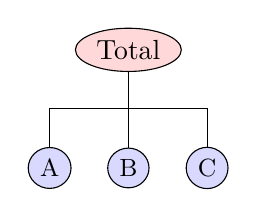
\begin{tikzpicture}
\tikzstyle{every node}=[ellipse,draw,fill=red!15,inner sep=2pt]
\tikzstyle[level distance=.3cm]
\tikzstyle[sibling distance=12cm]
\tikzstyle{level 1}=[sibling distance=10mm,font=\small,set style={{every node}+=[fill=blue!15]}]
\node{Total}[edge from parent fork down]
 child {node {A}
 }
 child {node {B}
 }
 child {node {C}
 };
\end{tikzpicture}
\end{block}
\end{minipage}
\end{textblock}

\begin{textblock}{5.7}(9.4,2.8)\fontsize{14}{15}\sf
\begin{align*}
\bY_{t}&= \begin{pmatrix}
  y_{\text{Total},t}\\
  y_{A,t}\\
  y_{B,t}\\
  y_{C,t}
  \end{pmatrix}  \\
  &= {\color{blue}\begin{pmatrix}
                1 & 1 & 1 \\
                1 & 0 & 0 \\
                0 & 1 & 0\\
                0 & 0 & 1
                \end{pmatrix}}
     {\color{red}\begin{pmatrix}
       y_{A,t}\\y_{B,t}\\y_{C,t}
       \end{pmatrix}}
\end{align*}
\end{textblock}
\end{frame}

\begin{frame}{The coherent subspace}
\phantomsection\label{the-coherent-subspace}
\begin{textblock}{9}(.2,1)\fontsize{13}{13}\sf
\begin{block}{Coherent subspace}
$n_b$-dimensional linear subspace $\mathfrak{s}\subset \mathbb{\chi}^n$ for which linear constraints hold for all $\bm{y}\in\mathfrak{s}$.
\end{block}\vspace*{-0.3cm}
\begin{block}{Hierarchical time series}
An $n$-dimensional multivariate time series such that $\bm{y}_t\in\mathfrak{s}\quad\forall t$.
\end{block}\vspace*{-0.3cm}
\begin{block}{Coherent point forecasts}
$\tilde{\bm{y}}_{t+h|t}$ is \emph{coherent} if $\tilde{\bm{y}}_{t+h|t} \in \mathfrak{s}$.
\end{block}\vspace*{-0.2cm}
\end{textblock}
\only<2-3>{\begin{textblock}{7.5}(.2,6.75)\fontsize{13}{13}\sf
\begin{alertblock}{Base forecasts}
Let $\hat{\bm{y}}_{t+h|t}$ be vector of \emph{incoherent} initial $h$-step forecasts.$\phantom{y_{t|h}}$
\end{alertblock}
\end{textblock}}
\only<3>{\begin{textblock}{7.5}(8.3,6.75)\fontsize{13}{13}\sf
\begin{alertblock}{Reconciled forecasts}
Let $\bm{M}$ be a projection matrix. $\tilde{\bm{y}}_{t+h|t}=\bm{M}\hat{\bm{y}}_{t+h|t}$ ``reconciles'' $\hat{\bm{y}}_{t+h|t}$.
\end{alertblock}
\end{textblock}}

\placefig{9.4}{.0}{width=6.6cm}{3D_hierarchy}
\begin{textblock}{3}(11.4,5.6)\fontsize{13}{13}\sf
\begin{block}{}
\centerline{$y_{Tot} = y_A + y_B$}
\end{block}
\end{textblock}
\end{frame}

\begin{frame}{Linear projection reconciliation}
\phantomsection\label{linear-projection-reconciliation}
\fontsize{14}{16}\sf
\vspace*{0.2cm}\begin{alertblock}{}
\centerline{$\tilde{\bm{y}}_{t+h|t}= \bm{M}\hat{\bm{y}}_{t+h|t}$}
\end{alertblock}\vspace*{-0.2cm}

\begin{itemize}
\tightlist
\item
  If \(\bm{S}\) forms a basis set for \(\mathfrak{s}\), then projections
  are of the form \(\bm{M} = \bS(\bS'\bm{\Psi}\bS)^{-1}\bS'\bm{\Psi}\)
  where \(\bm{\Psi}\) is a positive definite matrix.
\item
  Coherent base forecasts are unchanged since
  \(\bm{M}\hat{\bm{y}}=\hat{\bm{y}}\)
\item
  If \(\hat{\bm{y}}\) is unbiased, then \(\tilde{\bm{y}}\) is also
  unbiased.
\item
  \(\bm{W}_h = \var[\by_{T+h} - \hat{\by}_{T+h|T} \mid \by_1,\dots,\by_T]\)
  is the covariance matrix of the base forecast errors.
\item
  \(\bm{V}_h = \var[\by_{T+h} - \tilde{\by}_{T+h|T}  \mid \by_1,\dots,\by_T])  = \bm{M}\bm{W}_h\bm{M}'\)
  is the covariance matrix of the reconciled forecast errors.
\item
  How to choose the best \(\bm{\Psi}\)?
\end{itemize}

\vspace*{10cm}
\end{frame}

\begin{frame}{Minimum trace reconciliation}
\phantomsection\label{minimum-trace-reconciliation}
\begin{textblock}{6.4}(9,-0.1)\begin{block}{}
Wickramasuriya et al (2019)
\end{block}\end{textblock}

\vspace*{0.2cm}\begin{alertblock}{Minimum trace (MinT) reconciliation}
If $\bm{M}$ is a projection, then trace of $\bm{V}_h$ is minimized when $\bm{\Psi} = \bm{W}_h$, so that
\centerline{$\bm{M} = \bS(\bS'\bm{W}_h^{-1}\bS)^{-1}\bS'\bm{W}_h^{-1}$}
\end{alertblock}
\begin{block}{}
\centerline{$\displaystyle\textcolor{red}{\tilde{\by}_{T+h|T}}
= \bm{M} ~ \textcolor{blue}{\hat{\by}_{T+h|T}}$}
\end{block}\vspace*{-0.2cm}
\centerline{\hspace*{1.4cm}\textcolor{red}{Reconciled forecasts}\hfill\textcolor{blue}{Base forecasts}\hspace*{2.9cm}}\vspace*{-0.2cm}

\begin{itemize}
\tightlist
\item
  Trace of \(\bm{V}_h\) is sum of forecast variances.
\item
  MinT is \(L_2\) optimal amongst linear unbiased forecasts.
\item
  How to estimate
  \(\bm{W}_h = \var[\by_{T+h} - \hat{\by}_{T+h|T} \mid \by_1,\dots,\by_T]\)?
\end{itemize}
\end{frame}

\begin{frame}{Linear projections}
\phantomsection\label{linear-projections}
\begin{textblock}{5}(7,-0.2)
\begin{block}{}
\centerline{$\tilde{\by}_{T+h|T}=\bm{M}\hat{\by}_{T+h|T}$}
\end{block}
\end{textblock}

\begin{textblock}{9.4}(.5,1.2)
\begin{alertblock}{Reconciliation method \hspace*{0.5cm} $\bm{M}$}
\begin{tabular}{l@{\hspace*{-0.5cm}}l}
  OLS             & $\bS(\bS'\bS)^{-1}\bS'$ \\
  WLS(var)        & $\bS(\bS'\bm{\Lambda}_v\bS)^{-1}\bS'\bm{\Lambda}_v$ \\
  WLS(struct)     & $\bS(\bS'\bm{\Lambda}_s\bS)^{-1}\bS'\bm{\Lambda}_s$ \\
  MinT(sample)    & $\bS(\bS'\hat{\bm{W}}_{\text{sam}}^{-1}\bS)^{-1}\bS' \hat{\bm{W}}_{\text{sam}}^{-1}$  \\
  MinT(shrink)\hspace*{2cm}    & $(\bS'\hat{\bm{W}}_{\text{shr}}^{-1}\bS)^{-1}\bS' \hat{\bm{W}}_{\text{shr}}^{-1}$  \\
\end{tabular}
\end{alertblock}
\end{textblock}
\begin{textblock}{15}(.2,5.7)\fontsize{13}{15}\sf
\begin{itemize}\parskip=0cm
\item $\bm{\Lambda}_v = \text{diag}(\bm{W}_1)^{-1}$
\item $\bm{\Lambda}_s = \text{diag}(\bS\bm{1})^{-1}$
\item $\hat{\bm{W}}_{\text{sam}}$ is sample estimate of the residual covariance matrix
\item $\hat{\bm{W}}_{\text{shr}}$ is shrinkage estimator $\tau \text{diag}(\hat{\bm{W}}_{\text{sam}})+(1-\tau)\hat{\bm{W}}_{\text{sam}}$\\ where $\tau$ selected optimally.
\end{itemize}
\end{textblock}
\begin{textblock}{5}(10.3,3.35)
\begin{block}{}
These approximate MinT by assuming $\bm{W}_h = k_h \bm{W}_1$.
\end{block}
\end{textblock}
\end{frame}

\begin{frame}[fragile]{Example: Australian tourism}
\phantomsection\label{example-australian-tourism}
\fontsize{10}{11}\sf

\begin{Shaded}
\begin{Highlighting}[]
\NormalTok{tourism}
\end{Highlighting}
\end{Shaded}

\begin{verbatim}
# A tsibble: 69,312 x 6 [1M]
# Key:       state, zone, region, purpose [304]
      month state zone  region   purpose  visitors
      <mth> <chr> <chr> <chr>    <chr>       <dbl>
 1 1998 Jan NSW   ACT   Canberra Business     25.0
 2 1998 Feb NSW   ACT   Canberra Business    148. 
 3 1998 Mar NSW   ACT   Canberra Business    111. 
 4 1998 Apr NSW   ACT   Canberra Business     93.1
 5 1998 May NSW   ACT   Canberra Business     78.1
 6 1998 Jun NSW   ACT   Canberra Business     44.3
 7 1998 Jul NSW   ACT   Canberra Business    129. 
 8 1998 Aug NSW   ACT   Canberra Business     71.3
 9 1998 Sep NSW   ACT   Canberra Business     77.7
10 1998 Oct NSW   ACT   Canberra Business    145. 
# i 69,302 more rows
\end{verbatim}
\end{frame}

\begin{frame}[fragile]{Example: Australian tourism}
\phantomsection\label{example-australian-tourism-1}
\fontsize{10}{11}\sf

\begin{Shaded}
\begin{Highlighting}[]
\NormalTok{tourism\_agg }\OtherTok{\textless{}{-}}\NormalTok{ tourism }\SpecialCharTok{|\textgreater{}}
  \FunctionTok{aggregate\_key}\NormalTok{(state }\SpecialCharTok{/}\NormalTok{ zone }\SpecialCharTok{/}\NormalTok{ region, }\AttributeTok{visitors =} \FunctionTok{sum}\NormalTok{(visitors))}
\end{Highlighting}
\end{Shaded}

\begin{verbatim}
# A tsibble: 25,308 x 5 [1M]
# Key:       state, zone, region [111]
      month state        zone         region       visitors
      <mth> <chr*>       <chr*>       <chr*>          <dbl>
 1 1998 Jan <aggregated> <aggregated> <aggregated>   45151.
 2 1998 Feb <aggregated> <aggregated> <aggregated>   17295.
 3 1998 Mar <aggregated> <aggregated> <aggregated>   20725.
 4 1998 Apr <aggregated> <aggregated> <aggregated>   25389.
 5 1998 May <aggregated> <aggregated> <aggregated>   20330.
 6 1998 Jun <aggregated> <aggregated> <aggregated>   18238.
 7 1998 Jul <aggregated> <aggregated> <aggregated>   23005.
 8 1998 Aug <aggregated> <aggregated> <aggregated>   23033.
 9 1998 Sep <aggregated> <aggregated> <aggregated>   22483.
10 1998 Oct <aggregated> <aggregated> <aggregated>   24845.
# i 25,298 more rows
\end{verbatim}
\end{frame}

\begin{frame}[fragile]{Example: Australian tourism}
\phantomsection\label{example-australian-tourism-2}
\fontsize{10}{11}\sf

\begin{Shaded}
\begin{Highlighting}[]
\NormalTok{fit }\OtherTok{\textless{}{-}}\NormalTok{ tourism\_agg }\SpecialCharTok{|\textgreater{}}
  \FunctionTok{filter}\NormalTok{(}\FunctionTok{year}\NormalTok{(month) }\SpecialCharTok{\textless{}=} \DecValTok{2015}\NormalTok{) }\SpecialCharTok{|\textgreater{}}
  \FunctionTok{model}\NormalTok{(}\AttributeTok{ets =} \FunctionTok{ETS}\NormalTok{(visitors))}
\end{Highlighting}
\end{Shaded}

\begin{verbatim}
# A mable: 111 x 4
# Key:     state, zone, region [111]
   state  zone            region                   ets
   <chr*> <chr*>          <chr*>               <model>
 1 NSW    ACT             Canberra        <ETS(M,N,A)>
 2 NSW    ACT             <aggregated>    <ETS(M,N,A)>
 3 NSW    Metro NSW       Central Coast   <ETS(M,N,A)>
 4 NSW    Metro NSW       Sydney          <ETS(M,N,A)>
 5 NSW    Metro NSW       <aggregated>    <ETS(M,N,A)>
 6 NSW    North Coast NSW Hunter          <ETS(M,N,M)>
 7 NSW    North Coast NSW North Coast NSW <ETS(M,N,M)>
 8 NSW    North Coast NSW <aggregated>    <ETS(M,N,M)>
 9 NSW    North NSW       Blue Mountains  <ETS(M,N,M)>
10 NSW    North NSW       Central NSW     <ETS(A,N,A)>
# i 101 more rows
\end{verbatim}
\end{frame}

\begin{frame}[fragile]{Example: Australian tourism}
\phantomsection\label{example-australian-tourism-3}
\fontsize{10}{11}\sf

\begin{Shaded}
\begin{Highlighting}[]
\NormalTok{fc }\OtherTok{\textless{}{-}}\NormalTok{ fit }\SpecialCharTok{|\textgreater{}}
  \FunctionTok{reconcile}\NormalTok{(}
    \AttributeTok{ols =} \FunctionTok{min\_trace}\NormalTok{(ets, }\AttributeTok{method =} \StringTok{"ols"}\NormalTok{),}
    \AttributeTok{wlsv =} \FunctionTok{min\_trace}\NormalTok{(ets, }\AttributeTok{method =} \StringTok{"wls\_var"}\NormalTok{),}
    \AttributeTok{wlss =} \FunctionTok{min\_trace}\NormalTok{(ets, }\AttributeTok{method =} \StringTok{"wls\_struct"}\NormalTok{),}
    \CommentTok{\# mint\_c = min\_trace(ets, method="mint\_cov"),}
    \AttributeTok{mint\_s =} \FunctionTok{min\_trace}\NormalTok{(ets, }\AttributeTok{method =} \StringTok{"mint\_shrink"}\NormalTok{),}
\NormalTok{  ) }\SpecialCharTok{|\textgreater{}}
  \FunctionTok{forecast}\NormalTok{(}\AttributeTok{h =} \StringTok{"2 years"}\NormalTok{)}
\end{Highlighting}
\end{Shaded}

\begin{verbatim}
# A fable: 13,320 x 7 [1M]
# Key:     state, zone, region, .model [555]
   state  zone   region   .model    month      visitors .mean
   <chr*> <chr*> <chr*>   <chr>     <mth>        <dist> <dbl>
 1 NSW    ACT    Canberra ets    2016 Jan N(593, 21917)  593.
 2 NSW    ACT    Canberra ets    2016 Feb  N(367, 8384)  367.
 3 NSW    ACT    Canberra ets    2016 Mar N(461, 13247)  461.
 4 NSW    ACT    Canberra ets    2016 Apr N(506, 15968)  506.
 5 NSW    ACT    Canberra ets    2016 May N(430, 11509)  430.
 6 NSW    ACT    Canberra ets    2016 Jun  N(398, 9861)  398.
 7 NSW    ACT    Canberra ets    2016 Jul N(523, 17068)  523.
 8 NSW    ACT    Canberra ets    2016 Aug  N(392, 9564)  392.
 9 NSW    ACT    Canberra ets    2016 Sep N(442, 12153)  442.
10 NSW    ACT    Canberra ets    2016 Oct N(572, 20376)  572.
# i 13,310 more rows
\end{verbatim}
\end{frame}

\begin{frame}[fragile]{Example: Australian tourism}
\phantomsection\label{example-australian-tourism-4}
\fontsize{10}{11}\sf

\begin{Shaded}
\begin{Highlighting}[]
\NormalTok{fc }\SpecialCharTok{|\textgreater{}}
  \FunctionTok{filter}\NormalTok{(}\FunctionTok{is\_aggregated}\NormalTok{(state)) }\SpecialCharTok{|\textgreater{}}
  \FunctionTok{autoplot}\NormalTok{(}\FunctionTok{filter}\NormalTok{(tourism\_agg, }\FunctionTok{year}\NormalTok{(month) }\SpecialCharTok{\textgreater{}} \DecValTok{2012}\NormalTok{), }\AttributeTok{level =} \ConstantTok{NULL}\NormalTok{)}
\end{Highlighting}
\end{Shaded}

\includegraphics{subspace_projections_files/figure-beamer/fctourism2-1.pdf}
\end{frame}

\begin{frame}[fragile]{Example: Australian tourism}
\phantomsection\label{example-australian-tourism-5}
\fontsize{10}{11}\sf

\begin{Shaded}
\begin{Highlighting}[]
\NormalTok{fc }\SpecialCharTok{|\textgreater{}}
  \FunctionTok{filter}\NormalTok{(state }\SpecialCharTok{==} \StringTok{"NSW"} \SpecialCharTok{\&} \FunctionTok{is\_aggregated}\NormalTok{(zone)) }\SpecialCharTok{|\textgreater{}}
  \FunctionTok{autoplot}\NormalTok{(}\FunctionTok{filter}\NormalTok{(tourism\_agg, }\FunctionTok{year}\NormalTok{(month) }\SpecialCharTok{\textgreater{}} \DecValTok{2012}\NormalTok{), }\AttributeTok{level =} \ConstantTok{NULL}\NormalTok{)}
\end{Highlighting}
\end{Shaded}

\includegraphics{subspace_projections_files/figure-beamer/fctourism3-1.pdf}
\end{frame}

\begin{frame}[fragile]{Example: Australian tourism}
\phantomsection\label{example-australian-tourism-6}
\fontsize{10}{11}\sf

\begin{Shaded}
\begin{Highlighting}[]
\NormalTok{fc }\SpecialCharTok{|\textgreater{}}
  \FunctionTok{filter}\NormalTok{(region }\SpecialCharTok{==} \StringTok{"Melbourne"}\NormalTok{) }\SpecialCharTok{|\textgreater{}}
  \FunctionTok{autoplot}\NormalTok{(}\FunctionTok{filter}\NormalTok{(tourism\_agg, }\FunctionTok{year}\NormalTok{(month) }\SpecialCharTok{\textgreater{}} \DecValTok{2012}\NormalTok{), }\AttributeTok{level =} \ConstantTok{NULL}\NormalTok{)}
\end{Highlighting}
\end{Shaded}

\includegraphics{subspace_projections_files/figure-beamer/fctourism4-1.pdf}
\end{frame}

\begin{frame}[fragile]{Example: Australian tourism}
\phantomsection\label{example-australian-tourism-7}
\fontsize{10}{11}\sf

\begin{Shaded}
\begin{Highlighting}[]
\NormalTok{fc }\SpecialCharTok{|\textgreater{}}
  \FunctionTok{filter}\NormalTok{(region }\SpecialCharTok{==} \StringTok{"Snowy Mountains"}\NormalTok{) }\SpecialCharTok{|\textgreater{}}
  \FunctionTok{autoplot}\NormalTok{(}\FunctionTok{filter}\NormalTok{(tourism\_agg, }\FunctionTok{year}\NormalTok{(month) }\SpecialCharTok{\textgreater{}} \DecValTok{2012}\NormalTok{), }\AttributeTok{level =} \ConstantTok{NULL}\NormalTok{)}
\end{Highlighting}
\end{Shaded}

\includegraphics{subspace_projections_files/figure-beamer/fctourism5-1.pdf}
\end{frame}

\begin{frame}[fragile]{Example: Australian tourism}
\phantomsection\label{example-australian-tourism-8}
\fontsize{10}{11}\sf

\begin{Shaded}
\begin{Highlighting}[]
\NormalTok{fc }\SpecialCharTok{|\textgreater{}}
  \FunctionTok{filter}\NormalTok{(region }\SpecialCharTok{==} \StringTok{"Barossa"}\NormalTok{) }\SpecialCharTok{|\textgreater{}}
  \FunctionTok{autoplot}\NormalTok{(}\FunctionTok{filter}\NormalTok{(tourism\_agg, }\FunctionTok{year}\NormalTok{(month) }\SpecialCharTok{\textgreater{}} \DecValTok{2012}\NormalTok{), }\AttributeTok{level =} \ConstantTok{NULL}\NormalTok{)}
\end{Highlighting}
\end{Shaded}

\includegraphics{subspace_projections_files/figure-beamer/fctourism6-1.pdf}
\end{frame}

\begin{frame}{Performance evaluation}
\phantomsection\label{performance-evaluation}
\vspace*{0.2cm}\begin{block}{}
\centerline{$\text{MASE} = \text{mean}(|q_{j}|)$}
$$
  q_{j} = \frac{e_{j}\phantom{^2}}
 {\displaystyle\frac{1}{T-m}\sum_{t=m+1}^T |y_{t}-y_{t-m}|}
$$
\end{block}

\begin{itemize}
\tightlist
\item
  \(y_t=\) observation for period \(t\)
\item
  \(e_{j}=\) forecast error for forecast horizon \(j\)
\item
  \(T=\) size of training set
\item
  \(m = 12\)
\end{itemize}
\end{frame}

\begin{frame}{Performance evaluation}
\phantomsection\label{performance-evaluation-1}
\vspace*{0.2cm}\begin{block}{}
\centerline{$\text{RMSSE} = \sqrt{\text{mean}(q_{j}^2)}$}
$$
  q^2_{j} = \frac{ e^2_{j}}
 {\displaystyle\frac{1}{T-m}\sum_{t=m+1}^T (y_{t}-y_{t-m})^2}
$$
\end{block}

\begin{itemize}
\tightlist
\item
  \(y_t=\) observation for period \(t\)
\item
  \(e_{j}=\) forecast error for forecast horizon \(j\)
\item
  \(T=\) size of training set
\item
  \(m = 12\)
\end{itemize}
\end{frame}

\begin{frame}[fragile]{Example: Australian tourism}
\phantomsection\label{example-australian-tourism-9}
\fontsize{10}{11}\sf

\begin{Shaded}
\begin{Highlighting}[]
\NormalTok{fc }\SpecialCharTok{|\textgreater{}}
  \FunctionTok{accuracy}\NormalTok{(tourism\_agg, }\AttributeTok{measures =} \FunctionTok{list}\NormalTok{(}\AttributeTok{mase =}\NormalTok{ MASE, }\AttributeTok{rmsse =}\NormalTok{ RMSSE))}
\end{Highlighting}
\end{Shaded}

\begin{verbatim}
# A tibble: 555 x 7
   .model state  zone            region          .type  mase rmsse
   <chr>  <chr*> <chr*>          <chr*>          <chr> <dbl> <dbl>
 1 ets    NSW    ACT             Canberra        Test  0.546 0.513
 2 ets    NSW    ACT             <aggregated>    Test  0.546 0.513
 3 ets    NSW    Metro NSW       Central Coast   Test  0.909 0.829
 4 ets    NSW    Metro NSW       Sydney          Test  0.891 0.764
 5 ets    NSW    Metro NSW       <aggregated>    Test  0.848 0.715
 6 ets    NSW    North Coast NSW Hunter          Test  0.804 0.696
 7 ets    NSW    North Coast NSW North Coast NSW Test  1.21  1.17 
 8 ets    NSW    North Coast NSW <aggregated>    Test  1.10  0.986
 9 ets    NSW    North NSW       Blue Mountains  Test  0.932 1.13 
10 ets    NSW    North NSW       Central NSW     Test  1.02  0.805
# i 545 more rows
\end{verbatim}
\end{frame}

\begin{frame}[fragile]{Example: Australian tourism}
\phantomsection\label{example-australian-tourism-10}
\fontsize{10}{11}\sf

\begin{Shaded}
\begin{Highlighting}[]
\NormalTok{fc }\SpecialCharTok{|\textgreater{}}
  \FunctionTok{accuracy}\NormalTok{(tourism\_agg, }\AttributeTok{measures =} \FunctionTok{list}\NormalTok{(}\AttributeTok{mase =}\NormalTok{ MASE, }\AttributeTok{rmsse =}\NormalTok{ RMSSE)) }\SpecialCharTok{|\textgreater{}}
  \FunctionTok{group\_by}\NormalTok{(.model) }\SpecialCharTok{|\textgreater{}}
  \FunctionTok{summarise}\NormalTok{(}\AttributeTok{mase =} \FunctionTok{mean}\NormalTok{(mase), }\AttributeTok{rmsse =} \FunctionTok{sqrt}\NormalTok{(}\FunctionTok{mean}\NormalTok{(rmsse}\SpecialCharTok{\^{}}\DecValTok{2}\NormalTok{))) }\SpecialCharTok{|\textgreater{}}
  \FunctionTok{arrange}\NormalTok{(rmsse)}
\end{Highlighting}
\end{Shaded}

\begin{verbatim}
# A tibble: 5 x 3
  .model  mase rmsse
  <chr>  <dbl> <dbl>
1 ols    0.890 0.863
2 mint_s 0.878 0.866
3 wlss   0.886 0.871
4 wlsv   0.882 0.873
5 ets    0.886 0.880
\end{verbatim}

\only<2>{\begin{textblock}{7}(7,5)
\begin{block}{}\fontsize{13}{14}\sf
\begin{itemize}\tightlist
\item Overall, every reconciliation method is better than the base ETS forecasts.
\end{itemize}
\end{block}
\end{textblock}}
\end{frame}

\begin{frame}[fragile]{Example: Australian tourism}
\phantomsection\label{example-australian-tourism-11}
\fontsize{8}{7}\sf

\begin{verbatim}
# A tibble: 20 x 4
# Groups:   .model [5]
   .model level     mase rmsse
   <chr>  <fct>    <dbl> <dbl>
 1 ets    National 0.806 0.755
 2 ols    National 0.812 0.768
 3 wlss   National 0.846 0.889
 4 mint_s National 0.853 0.896
 5 wlsv   National 0.883 0.934
 6 ols    State    0.902 0.905
 7 ets    State    0.921 0.919
 8 mint_s State    0.956 0.953
 9 wlss   State    0.950 0.954
10 wlsv   State    0.966 0.971
11 ols    Zone     0.932 0.912
12 mint_s Zone     0.924 0.914
13 wlss   Zone     0.931 0.924
14 wlsv   Zone     0.933 0.925
15 ets    Zone     0.936 0.935
16 mint_s Region   0.855 0.839
17 ols    Region   0.875 0.843
18 wlsv   Region   0.856 0.843
19 wlss   Region   0.864 0.844
20 ets    Region   0.866 0.858
\end{verbatim}

\only<2>{\begin{textblock}{7}(7,5)
\begin{block}{}\fontsize{13}{14}\sf
\begin{itemize}\tightlist
\item OLS is best for all levels except national.
\item Improvements due to reconciliation are greater at lower levels.
\end{itemize}
\end{block}
\end{textblock}}
\end{frame}

\begin{frame}{Mean square error bounds}
\phantomsection\label{mean-square-error-bounds}
\begin{textblock}{6.4}(9,-0.1)\begin{block}{}
\citet{htsgeometry}
\end{block}\end{textblock}

\vspace*{0.2cm}\begin{alertblock}{Distance reducing property}
Let $\|\bm{u}\|_{\bm{\Psi}} = \bm{u}'\bm{\Psi}\bm{u}$. Then
  \centerline{$\|\bm{y}_{t+h}-\tilde{\bm{y}}_{t+h|t}\|_{\bm{\Psi}}\le\|\bm{y}_{t+h}-\hat{\bm{y}}_{t+h|t}\|_{\bm{\Psi}}$}
\end{alertblock}

\begin{itemize}
\tightlist
\item
  \(\bm{\Psi}\)-projection is guaranteed to improve forecast accuracy
  over base forecasts \emph{using this distance measure}.
\item
  Distance reduction holds for any realisation and any forecast.
\item
  OLS reconciliation minimizes Euclidean distance.
\end{itemize}
\end{frame}

\begin{frame}{Mean square error bounds}
\phantomsection\label{mean-square-error-bounds-1}
\begin{textblock}{6.4}(9,-0.1)\begin{block}{}
\citet{wickramasuriya2021properties}
\end{block}\end{textblock}

\begin{block}{}\vspace*{-0.6cm}
\begin{align*}
\|\bm{y}_{t+h} - \tilde{\bm{y}}_{t+h}\|_2^2
 &= \|\bm{M}(\bm{y}_{t+h} - \hat{\bm{y}}_{t+h})\|_2^2 \\
 &\le \|\bm{M}\|_2^2 \|\bm{y}_{t+h} - \hat{\bm{y}}_{t+h}\|_2^2 \\
 & = \sigma_{\text{max}}^2\|\bm{y}_{t+h} - \hat{\bm{y}}_{t+h}\|_2^2
\end{align*}
\end{block}

\begin{itemize}
\tightlist
\item
  \(\sigma_{\text{max}}\) is the largest eigenvalue of \(\bm{M}\)
\item
  \(\sigma_{\text{max}}\ge1\) as \(\bm{M}\) is a projection matrix.
\item
  Every projection reconciliation is better than base forecasts using
  Euclidean distance.
\end{itemize}
\end{frame}

\begin{frame}{Mean square error bounds}
\phantomsection\label{mean-square-error-bounds-2}
\begin{textblock}{6.4}(9,-0.1)\begin{block}{}
\citet{wickramasuriya2021properties}
\end{block}\end{textblock}
\vspace*{0.2cm}\begin{block}{}\vspace*{-0.6cm}
\begin{align*}
    & \text{tr}\Big(\E[\bm{y}_{t+h} - \tilde{\bm{y}}^{\text{MinT}}_{t+h|t}]'[\bm{y}_{t+h} - \tilde{\bm{y}}^{\text{MinT}}_{t+h|t}]\Big) \\
\le~ & \text{tr}\Big(\E[\bm{y}_{t+h} - \tilde{\bm{y}}^{\text{OLS}}_{t+h|t}]'[\bm{y}_{t+h} - \tilde{\bm{y}}^{\text{OLS}}_{t+h|t}]\Big) \\
\le~ & \text{tr}\Big(\E[\bm{y}_{t+h} - \hat{\bm{y}}_{t+h|t}]'[\bm{y}_{t+h} - \hat{\bm{y}}_{t+h|t}]\Big)
\end{align*}
\end{block}

Using sums of variances:

\begin{itemize}
\tightlist
\item
  MinT reconciliation is better than OLS reconciliation
\item
  OLS reconciliation is better than base forecasts
\end{itemize}
\end{frame}

\section{Improving univariate
forecasts}\label{improving-univariate-forecasts}

\begin{frame}{Temporal reconciliation: quarterly data}
\phantomsection\label{temporal-reconciliation-quarterly-data}
\begin{textblock}{7}(1,1.9)
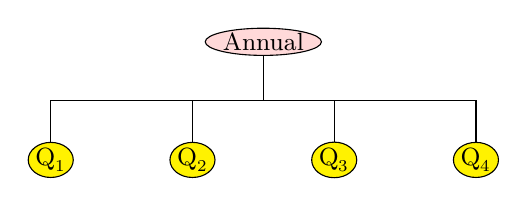
\begin{tikzpicture}
  \tikzstyle{every node}=[ellipse,draw,inner sep=0.2pt,fill=red!15,font=\small]
  \tikzstyle[level distance=.1cm]
  \tikzstyle[sibling distance=3cm]
  \tikzstyle{level 1}=[sibling distance=18mm,set style={{every node}+=[fill=yellow]}]
  \node{Annual}[edge from parent fork down]
  child {node {Q$_1$}}
  child {node {Q$_2$}}
  child {node {Q$_3$}}
  child {node {Q$_4$}};
\end{tikzpicture}
\end{textblock}

\only<3>{\begin{textblock}{8.5}(8.3,1.1)\fontsize{14}{17}\sf
$$\bm{y}_\tau =
  \begin{bmatrix}
    x_{\tau}^{[4]}  \\[0.2cm]
    x_{\tau,1}^{[1]} \\[0.2cm]
    x_{\tau,2}^{[1]} \\[0.2cm]
    x_{\tau,3}^{[1]} \\[0.2cm]
    x_{\tau,4}^{[1]}
  \end{bmatrix}
  \qquad
  \bm{S} = \begin{bmatrix}
    1 & 1 & 1 & 1 \\[0.2cm]
    1 & 0 & 0 & 0 \\[0.2cm]
    0 & 1 & 0 & 0 \\[0.2cm]
    0 & 0 & 1 & 0 \\[0.2cm]
    0 & 0 & 0 & 1
  \end{bmatrix}
$$
\end{textblock}}

\only<2->{\begin{textblock}{8}(.3,5.7)
  \begin{alertblock}{}
    \begin{itemize}
      \item[\color{white}\ding{229}] Forecast series at each available frequency.
      \item[\color{white}\ding{229}] Optimally combine forecasts within the same year.
    \end{itemize}
  \end{alertblock}
\end{textblock}}

\only<3->{\begin{textblock}{5}(10.3,7.9)
\fontsize{11}{12}\sf
$\tau=$ index of largest temporal aggregation level.
\end{textblock}}
\end{frame}

\begin{frame}{Temporal reconciliation: quarterly data}
\phantomsection\label{temporal-reconciliation-quarterly-data-1}
\begin{textblock}{7}(0.1,1.9)
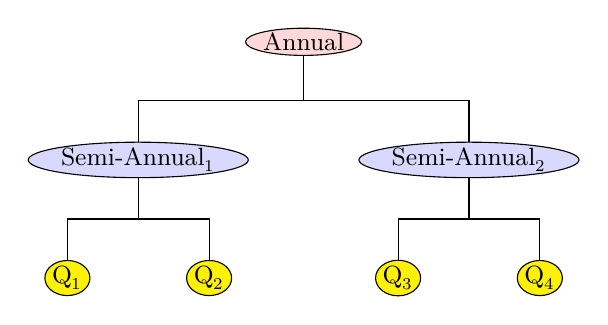
\begin{tikzpicture}
  \tikzstyle{every node}=[ellipse,draw,inner sep=0.2pt,fill=red!15,font=\small]
  \tikzstyle[level distance=.1cm]
  \tikzstyle[sibling distance=3cm]
  \tikzstyle{level 1}=[sibling distance=42mm,set style={{every node}+=[fill=blue!15]}]
  \tikzstyle{level 2}=[sibling distance=18mm,set style={{every node}+=[fill=yellow]}]
  \node{Annual}[edge from parent fork down]
  child {node {Semi-Annual$_1$}
      child {node {Q$_1$}}
      child {node {Q$_2$}}
    }
  child {node {Semi-Annual$_2$}
      child {node {Q$_3$}}
      child {node {Q$_4$}}
    };
\end{tikzpicture}
\end{textblock}

\begin{textblock}{8.5}(8.3,1.1)\fontsize{14}{17}\sf
$$\bm{y}_\tau =
  \begin{bmatrix}
    x_{\tau}^{[4]}  \\[0.2cm]
    x_{\tau,1}^{[2]} \\[0.2cm]
    x_{\tau,2}^{[2]} \\[0.2cm]
    x_{\tau,1}^{[1]} \\[0.2cm]
    x_{\tau,2}^{[1]} \\[0.2cm]
    x_{\tau,3}^{[1]} \\[0.2cm]
    x_{\tau,4}^{[1]}
  \end{bmatrix}
  \qquad
  \bm{S} = \begin{bmatrix}
    1 & 1 & 1 & 1 \\[0.2cm]
    1 & 1 & 0 & 0 \\[0.2cm]
    0 & 0 & 1 & 1 \\[0.2cm]
    1 & 0 & 0 & 0 \\[0.2cm]
    0 & 1 & 0 & 0 \\[0.2cm]
    0 & 0 & 1 & 0 \\[0.2cm]
    0 & 0 & 0 & 1
  \end{bmatrix}
$$
\end{textblock}

\begin{textblock}{8}(.3,5.7)
  \begin{alertblock}{}
    \begin{itemize}
      \item[\color{white}\ding{229}] Forecast series at each available frequency.
      \item[\color{white}\ding{229}] Optimally combine forecasts within the same year.
    \end{itemize}
  \end{alertblock}
\end{textblock}

\begin{textblock}{5}(10.3,7.9)
\fontsize{11}{12}\sf
$\tau=$ index of largest temporal aggregation level.
\end{textblock}
\end{frame}

\begin{frame}{Temporal reconciliation: monthly data}
\phantomsection\label{temporal-reconciliation-monthly-data}
\only<1>{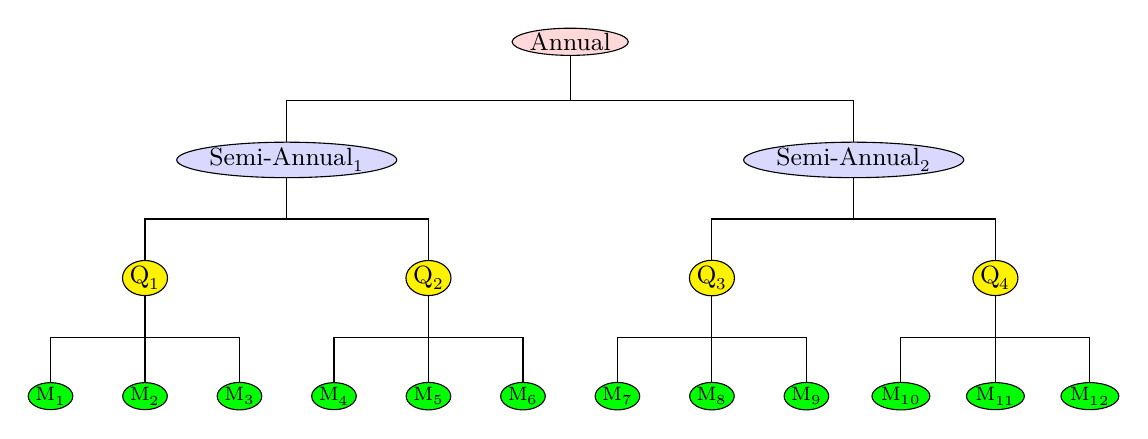
\begin{tikzpicture}
  \tikzstyle{every node}=[ellipse,draw,inner sep=0.2pt,fill=red!15,font=\small]
  \tikzstyle[level distance=.1cm]
  \tikzstyle[sibling distance=7cm]
  \tikzstyle{level 1}=[sibling distance=72mm,set style={{every node}+=[fill=blue!15]}]
  \tikzstyle{level 2}=[sibling distance=36mm,set style={{every node}+=[fill=yellow]}]
  \tikzstyle{level 3}=[sibling distance=12mm,font=\scriptsize,set style={{every node}+=[fill=green]}]
  \node{Annual}[edge from parent fork down]
  child {node {Semi-Annual$_1$}
      child {node {Q$_1$}
          child {node {\scriptsize M$_1$}}
          child {node {\scriptsize M$_2$}}
          child {node {\scriptsize M$_3$}}
        }
      child {node {Q$_2$}
          child {node {\scriptsize M$_4$}}
          child {node {\scriptsize M$_5$}}
          child {node {\scriptsize M$_6$}}
        }
    }
  child {node {Semi-Annual$_2$}
      child {node {Q$_3$}
          child {node {\scriptsize M$_7$}}
          child {node {\scriptsize M$_8$}}
          child {node {\scriptsize M$_9$}}
        }
      child {node {Q$_4$}
          child {node {\scriptsize M$_{10}$}}
          child {node {\scriptsize M$_{11}$}}
          child {node {\scriptsize M$_{12}$}}
        }
    };
\end{tikzpicture}}
\only<2->{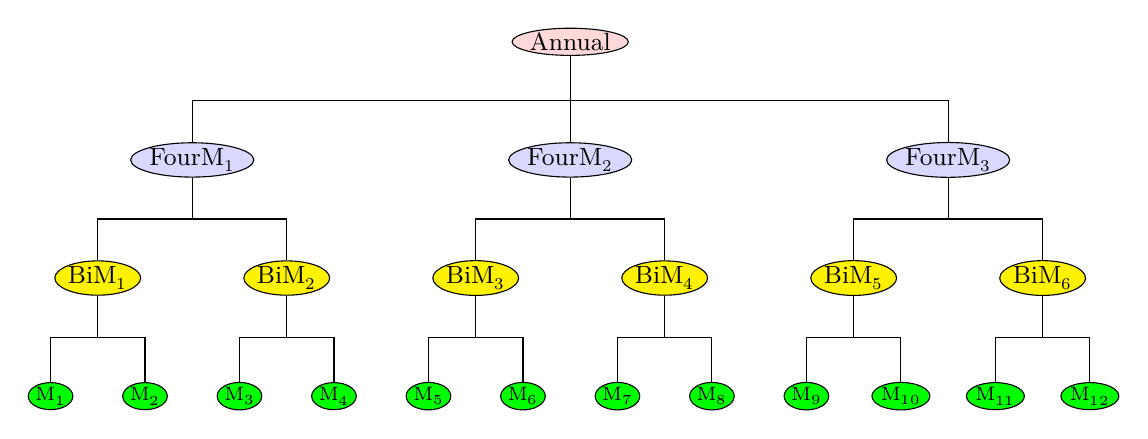
\begin{tikzpicture}
  \tikzstyle{every node}=[ellipse,draw,inner sep=0.2pt,fill=red!15,font=\small]
  \tikzstyle[level distance=.1cm]
  \tikzstyle[sibling distance=7cm]
  \tikzstyle{level 1}=[sibling distance=48mm,set style={{every node}+=[fill=blue!15]}]
  \tikzstyle{level 2}=[sibling distance=24mm,set style={{every node}+=[fill=yellow]}]
  \tikzstyle{level 3}=[sibling distance=12mm,set style={{every node}+=[fill=green]}]
  \node{Annual}[edge from parent fork down]
  child {node {FourM$_1$}
      child {node {BiM$_1$}
          child {node {\scriptsize M$_1$}}
          child {node {\scriptsize M$_2$}}
        }
      child {node {BiM$_2$}
          child {node {\scriptsize M$_3$}}
          child {node {\scriptsize M$_4$}}
        }
    }
  child {node {FourM$_2$}
      child {node {BiM$_3$}
          child {node {\scriptsize M$_5$}}
          child {node {\scriptsize M$_6$}}
        }
      child {node {BiM$_4$}
          child {node {\scriptsize M$_7$}}
          child {node {\scriptsize M$_8$}}
        }
    }
  child {node {FourM$_3$}
      child {node {BiM$_5$}
          child {node {\scriptsize M$_9$}}
          child {node {\scriptsize M$_{10}$}}
        }
      child {node {BiM$_6$}
          child {node {\scriptsize M$_{11}$}}
          child {node {\scriptsize M$_{12}$}}
        }
    };
\end{tikzpicture}}\pause

\begin{textblock}{14}(1,6.7)
  \begin{alertblock}{}
    \begin{itemize}
      \item[\color{white}\ding{229}] Forecast series at each available frequency.
      \item[\color{white}\ding{229}] Optimally combine forecasts within the same year.
    \end{itemize}
  \end{alertblock}
\end{textblock}
\end{frame}

\begin{frame}{Temporal reconciliation: monthly data}
\phantomsection\label{temporal-reconciliation-monthly-data-1}
\fontsize{11}{11}\sf

\[
  \bm{y}_\tau=\begin{bmatrix}
    x_{\tau}^{[12]}     \\[0.2cm]
    \bm{x}_{\tau}^{[6]} \\[0.2cm]
    \bm{x}_{\tau}^{[4]} \\[0.2cm]
    \bm{x}_{\tau}^{[3]} \\[0.2cm]
    \bm{x}_\tau^{[2]}   \\[0.2cm]
    \bm{x}_\tau^{[1]}
  \end{bmatrix}
  \qquad
  \bm{S} = \begin{bmatrix}
    1                & 1 & 1 & 1 & 1~~~1~~~1~~~1 & 1 & 1 & 1 & 1 \\
    1                & 1 & 1 & 1 & 1~~~1~~~0~~~0 & 0 & 0 & 0 & 0 \\
    0                & 0 & 0 & 0 & 0~~~0~~~1~~~1 & 1 & 1 & 1 & 1 \\
    1                & 1 & 1 & 1 & 0~~~0~~~0~~~0 & 0 & 0 & 0 & 0 \\
    0                & 0 & 0 & 0 & 1~~~1~~~1~~~1 & 0 & 0 & 0 & 0 \\
    0                & 0 & 0 & 0 & 0~~~0~~~0~~~0 & 1 & 1 & 1 & 1 \\
    1                & 1 & 1 & 0 & 0~~~0~~~0~~~0 & 0 & 0 & 0 & 0 \\
                     &   &   &   & \vdots        &   &   &   &   \\
    0                & 0 & 0 & 0 & 0~~~0~~~0~~~0 & 0 & 1 & 1 & 1 \\
    1                & 1 & 0 & 0 & 0~~~0~~~0~~~0 & 0 & 0 & 0 & 0 \\
                     &   &   &   & \vdots        &   &   &   &   \\
    0                & 0 & 0 & 0 & 0~~~0~~~0~~~0 & 0 & 0 & 1 & 1 \\[0.2cm]
    \phantom{\vdots} &   &   &   & \bm{I}_{12}   &   &   &   &
  \end{bmatrix}
\]
\end{frame}

\begin{frame}{Temporal reconciliation}
\phantomsection\label{temporal-reconciliation}
\fontsize{14}{15}\sf

For a time series \(y_1,\dots,y_T\), observed at frequency \(m\):

\begin{alertblock}{}\vspace*{-0.1cm}
$$
  x_j^{[k]} = \sum_{t = (j-1)k+1}^{jk} y_t\qquad \text{for $j = 1,\dots,\lfloor T/k\rfloor$}
$$
\end{alertblock}

\begin{itemize}
\tightlist
\item
  \(k \in \mathcal{K} = \{k_1,\dots,k_p\}\) denote the \(p\) factors of
  \(m\) in ascending order, where \(k_1=1\) and \(k_p=m\)
\item
  \(x_j^{[1]} = y_t\)
\item
  A single unique hierarchy is only possible when there are no coprime
  pairs in \(\mathcal{K}\).
\item
  \(M_k=m/k\) is seasonal period of aggregated series.
\end{itemize}
\end{frame}

\begin{frame}{Temporal reconciliation}
\phantomsection\label{temporal-reconciliation-1}
\fontsize{14}{15}\sf\vspace*{-0.5cm}

\[\bm{x}_\tau = \bm{S} \bm{x}_\tau^{[1]}, \qquad \bm{S} = \begin{bmatrix}\bm{A}\\\bm{I}\end{bmatrix}\]
where \[
\bm{x}_\tau = \begin{bmatrix*}[l]
    {x_\tau^{[k_p]}}\\
    {\bm{x}_\tau^{[k_{p-1}]}}\\
    \quad\vdots\\
    {\bm{x}_\tau^{[k_1]}}\\
  \end{bmatrix*}\qquad
  \bm{x}_\tau^{[k]} = \begin{bmatrix*}[l]
    x_{M_k(\tau-1)+1}^{[k]}\\
    x_{M_k(\tau-1)+2}^{[k]}\\
    \quad\vdots\\
    x_{M_k\tau}^{[k]}
  \end{bmatrix*}\qquad
\bm{A} =
  \begin{bmatrix}
    \bm{1}'_m                                    \\
    \bm{I}_{m/k_{p-1}} \otimes \bm{1}'_{k_{p-1}} \\
    \vdots                                       \\
    \bm{I}_{m/k_{2}} \otimes \bm{1}'_{k_{2}}     \\
  \end{bmatrix}
\] \(\tau\) is time index for most aggregated series,

\(k\in \mathcal{K} = \{k_1,\dots,k_p\}\),\quad \(k_1=1\),\quad \(k_p=m\),\quad \(\tau=1,\dots,T/m\).
\end{frame}

\begin{frame}{Monthly Australian Tourism Demand}
\phantomsection\label{monthly-australian-tourism-demand}
\only<1>{\placefig{0.1}{1.3}{width=15.8cm}{tourism7}}
\only<2>{\placefig{0.1}{1.3}{width=15.8cm}{tourism8}}
\end{frame}

\begin{frame}{Monthly Australian Tourism Demand}
\phantomsection\label{monthly-australian-tourism-demand-1}
\begin{textblock}{6}(0.2,1.2)
\centering\fontsize{12}{13}\sf
\textbf{Geographical division}\\
\includegraphics[width = 5.5cm, trim= 0 0 180 0, clip=true]{subspace_projections_files/figure-beamer/ausmap-1.pdf}\\[-0.4cm]
\faTimes\\
\textbf{Purpose of travel}\\
{\fontsize{11}{12}\sf Holiday, Visiting friends \& relatives, Business, Other}
\end{textblock}

\begin{textblock}{10}(6.1,1)
\fontsize{11}{14}\sf\tabcolsep=0.12cm
\begin{itemize}
\item \textbf{Grouped ts}\newline (geographical divisions $\times$ purpose of travel)

\begin{tabular}{lccccc}
\toprule
  & \textbf{AUS} & \textbf{States} & \textbf{Zones$^\ast$} & \textbf{Regions} & \textbf{Tot}\\
  \midrule
  \textbf{geographical} & {\color{newblue}1} & {\color{newblue}7} & {\color{newblue}21} & {\color{newblue}76} & 105 \\
  \textbf{purpose} & {\color{newblue}4} & {\color{newblue}28} & {\color{newblue}84} & {\color{avocado}304} & 420\\
  \midrule
  \textbf{total} & 5 & 35 & 105 & 380 & \textbf{525}\\
  \bottomrule
\end{tabular}
\centerline{{\color{newblue}$n_a = 221$}, {\color{avocado}$n_b = 304$}, and $\textbf{n = 525}$}

\item \textbf{Temporal framework}, frequencies:\\[0.2cm]
\begin{multicols}{2}
  \begin{itemize}\tightlist
  \item Monthly
  \item Bi-Monthly
  \item Quarterly
  \end{itemize}
  \begin{itemize}\tightlist
  \item Four-Monthly
  \item Semi-Annual
  \item Annual
  \end{itemize}
\end{multicols}
\end{itemize}
\end{textblock}
\end{frame}

\begin{frame}{Monthly Australian Tourism Demand}
\phantomsection\label{monthly-australian-tourism-demand-2}
\begin{itemize}
\item
  Monthly data: January 1998 to December 2016
\item
  Time series cross-validation; initial training set 10 years.
\item
  One-month increase in each training set
\item
  For each training set, compute temporally aggregated series for
  \(k \in \{1,2,3,4,6,12\}\), and produce forecasts up to \(h_2=6\),
  \(h_3=4\), \(h_4=3\), \(h_6=2\) and \(h_{12}=1\) steps ahead.
\item
  Automatic ETS forecasts on log-transformed data
\end{itemize}
\end{frame}

\section{Improving multivariate
forecasts}\label{improving-multivariate-forecasts}

\section{Final comments}\label{final-comments}

\begin{frame}[fragile]{Software}
\phantomsection\label{software}
\fontsize{11}{12}\sf\vspace*{0.3cm}

\hspace*{-0.6cm}\begin{tabular}{llP{1.7cm}cP{1.7cm}c}
\toprule
Package                                                                      & Language  & Cross-sectional  & Temporal    & Cross-temporal  & Probabilistic\\
\midrule
\texttt{\href{https://pkg.earo.me/hts/}{hts}}
    & R         & \checkmark       &             &                 & \\
\texttt{\href{http://pkg.robjhyndman.com/thief/}{thief}}
    & R         &                  & \checkmark  &                 & \\
\texttt{\href{https://fable.tidyverts.org}{fable}}
    & R         & \checkmark       &             &                 & \checkmark\\
\texttt{\href{https://danigiro.github.io/FoReco/}{FoReco}}
    & R         & \checkmark       & \checkmark  & \checkmark      & \checkmark\\
\texttt{\href{https://angelpone.github.io/pyhts/}{pyhts}}
    & Python    & \checkmark       & \checkmark  &                 & \\
\texttt{\href{https://nixtla.github.io/hierarchicalforecast/}{hierarchicalforecast}}
    & Python    & \checkmark       &             &                 & \checkmark \\
\bottomrule
\end{tabular}

\begin{itemize}
\tightlist
\item
  \texttt{hts}, \texttt{thief}, and \texttt{FoReco} use \texttt{ts}
  objects
\item
  \texttt{fable} uses \texttt{tsibble} objects
\item
  \texttt{fable} has plans to implement temporal and cross-temporal
  reconciliation
\end{itemize}
\end{frame}

\begin{frame}{Thanks!}
\phantomsection\label{thanks}
\placefig{0}{1.2}{trim = 10 45 0 0, clip=TRUE, width=10cm, height=2.5cm}{roman}
\placefig{2}{1.2}{trim = 0 40 0 0, clip=TRUE, width=10cm, height=2.5cm}{george}
\placefig{4}{1.2}{trim = 0 10 0 0, clip=TRUE, width=10cm, height=2.5cm}{hanlin}
\placefig{6}{1.2}{trim = 10 0 0 0, clip=TRUE, width=10cm, height=2.5cm}{earowang}
\placefig{8}{1.2}{trim = 0 15 0 0, clip=TRUE, width=10cm, height=2.5cm}{alanlee}
\placefig{10}{1.2}{trim = 30 0 0 0, clip=TRUE, width=10cm, height=2.5cm}{mitch}
\placefig{12}{1.2}{trim = 15 0 0 0, clip=TRUE, width=10cm, height=2.5cm}{shanika}
\placefig{14}{1.2}{trim = 40 0 0 0, clip=TRUE, width=10cm, height=2.5cm}{tas}

\placefig{0}{3.8}{trim = 30 10 30 0, clip=TRUE, width=10cm, height=2.5cm}{puwasala}
\placefig{2}{3.8}{trim = 0 10 0 0, clip=TRUE, width=10cm, height=2.5cm}{fotios}
\placefig{4}{3.8}{trim = 100 30 50 20, clip=TRUE, width=10cm, height=2.5cm}{nikos}
\placefig{6}{3.8}{trim = 50 30 0 0, clip=TRUE, width=10cm, height=2.5cm}{souhaib}
\placefig{8}{3.8}{trim = 110 40 50 0, clip=TRUE, width=10cm, height=2.5cm}{james}
\placefig{10}{3.8}{trim = 40 40 0 0, clip=TRUE, width=10cm, height=2.5cm}{mahdi}
\placefig{12}{3.8}{trim = 50 50 0 0, clip=TRUE, width=10cm, height=2.5cm}{christoph}
\placefig{14}{3.8}{trim = 50 50 0 20, clip=TRUE, width=10cm, height=2.5cm}{fin}

\placefig{0}{6.4}{trim = 10 0 0 0, clip=TRUE, width=10cm, height=2.5cm}{berwin}
\placefig{2}{6.4}{trim = 10 20 0 0, clip=TRUE, width=10cm, height=2.5cm}{galit}
\placefig{4}{6.4}{trim = 10 0 0 0, clip=TRUE, width=10cm, height=2.5cm}{mahsa}
\placefig{6}{6.4}{trim = 30 0 0 0, clip=TRUE, width=10cm, height=2.5cm}{evan}
\placefig{8}{6.4}{trim = 5 25 0 0, clip=TRUE, width=10cm, height=2.5cm}{bahman}
\placefig{10}{6.4}{trim = 0 40 0 0, clip=TRUE, width=10cm, height=2.5cm}{pablo}
\placefig{12}{6.4}{trim = 0 40 0 0, clip=TRUE, width=10cm, height=2.5cm}{danielegiro}
\placefig{14}{6.4}{trim = 0 0 0 30, clip=TRUE, width=10cm, height=2.5cm}{tommy}
\end{frame}

\begin{frame}{More information}
\phantomsection\label{more-information}
\fontsize{18}{20}\sf

\href{https://robjhyndman.com}{\faicon{home} robjhyndman.com}

\href{https://aus.social/@robjhyndman}{
\includegraphics[width=0.5cm]{figs/mastodon}\, aus.social/@robjhyndman}

\href{https://github.com/robjhyndman}{\faicon{github}  @robjhyndman}

\href{mailto:rob.hyndman@monash.edu}{\faicon{envelope}  rob.hyndman@monash.edu}

\nocite{Di_FonGir2022a,temporal-hierarchies,ctprob}
\end{frame}


\begin{frame}[allowframebreaks]{}
  \bibliographytrue
  \printbibliography[heading=none]
\end{frame}



\end{document}
